\documentclass[12pt]{article}
\usepackage[spanish]{babel}
\usepackage{natbib}
\usepackage{url}
\usepackage[utf8x]{inputenc}
\usepackage{amsmath}
\usepackage{hyperref}
\usepackage[style=listgroup,acronym,toc,hyperfirst,xindy]{glossaries}
\makeglossaries
\usepackage[xindy]{imakeidx}
\makeindex
\usepackage{wrapfig}
\usepackage{graphicx}
\graphicspath{{images/}}
\usepackage{parskip}
\usepackage{fancyhdr}
\usepackage{vmargin}
\setmarginsrb{3 cm}{2.5 cm}{3 cm}{2.5 cm}{1 cm}{1.5 cm}{1 cm}{1.5 cm}

\setglossarystyle{long}

\newacronymstyle{ex-footnote}%
{%
	\GlsUseAcrEntryDispStyle{footnote}%
}%
{%
	\GlsUseAcrStyleDefs{footnote}%
	\renewcommand*{\genacrfullformat}[2]{%
		\firstacronymfont{\glsentryshort{##1}}##2%
		\expandafter\footnote\expandafter{\expandafter\glsentrylong\expandafter{##1}}%
	}%
	\renewcommand*{\Genacrfullformat}[2]{%
		\firstacronymfont{\Glsentryshort{##1}}##2%
		\expandafter\footnote\expandafter{\expandafter\glsentrylong\expandafter{##1}}%
	}%
	\renewcommand*{\genplacrfullformat}[2]{%
		\firstacronymfont{\glsentryshortpl{##1}}##2%
		\expandafter\footnote\expandafter{\expandafter\glsentrylongpl\expandafter{##1}}%
	}%
	\renewcommand*{\Genplacrfullformat}[2]{%
		\firstacronymfont{\Glsentryshortpl{##1}}##2%
		\expandafter\footnote\expandafter{\expandafter\glsentrylongpl\expandafter{##1}}%
	}%
}

\setacronymstyle{ex-footnote}



%Glossary
\newglossaryentry{vhfg}
{
	name=VFH,
	description={Banda del espectro electromagnético que ocupa el rango de frecuencias de 30 MHz a 300 MHz}
}
\newglossaryentry{uhfg}
{
	name=UFH,
	description={Banda del espectro electromagnético que ocupa el rango de frecuencias de 300 MHz a 3 GHz}
}

% Acronym list
\newacronym{oscar}{OSCAR}{Orbiting Satellite Carrying Amateur Radio}
\newacronym[see={[Glossary:]{vhfg}}]{vhf}{VHF}{Very High Frequency}
\newacronym[see={[Glossary:]{uhfg}}]{uhf}{UHF}{Ultra High Frequency}
\newacronym{satnogs}{SatNOGS}{Satellite Networked Operation Ground Stations}


\title{Diseño de una antena helicoidal \\para radioenlace satelital en UHF}								% Title
\author{Alberto Mur López \\ Diego Cajal Orleans}								% Author
\date{\today}											% Date

\makeatletter
\let\thetitle\@title
\let\theauthor\@author
\let\thedate\@date
\makeatother

\pagestyle{fancy}
\fancyhf{}
\rhead{\theauthor}
\lhead{\thetitle}
\cfoot{\thepage}

\begin{document}

%%%%%%%%%%%%%%%%%%%%%%%%%%%%%%%%%%%%%%%%%%%%%%%%%%%%%%%%%%%%%%%%%%%%%%%%%%%%%%%%%%%%%%%%%

\begin{titlepage}
	\centering
    \vspace*{0.5 cm}
    
\includegraphics[scale = 0.75]{eina.png}\\[1.0 cm]	% University Logo
%    \textsc{\LARGE University of Cape Town}\\[2.0 cm]	% University Name
	\textsc{\Large 30340}\\[0.5 cm]				% Course Code
	\textsc{\large equipos y sistemas de transmisión}\\[0.5 cm]				% Course Name
	\rule{\linewidth}{0.2 mm} \\[0.4 cm]
	\setlength{\baselineskip}{2\baselineskip}
	{ \huge \bfseries \thetitle}\\
	\rule{\linewidth}{0.2 mm} \\[1.5 cm]
	
	\begin{minipage}{0.4\textwidth}
		\begin{flushleft} \large
			\emph{Autores:}\\
			\theauthor
			\end{flushleft}
			\end{minipage}~
			\begin{minipage}{0.4\textwidth}
			\begin{flushright} \large
			\emph{Nia:} \\
			565825 \\
			658212
												% Your Student Number
		\end{flushright}
	\end{minipage}\\[2 cm]
	
	{\large \thedate}\\[2 cm]
 
	\vfill
	
\end{titlepage}

%%%%%%%%%%%%%%%%%%%%%%%%%%%%%%%%%%%%%%%%%%%%%%%%%%%%%%%%%%%%%%%%%%%%%%%%%%%%%%%%%%%%%%%%%

\tableofcontents
\pagebreak

%%%%%%%%%%%%%%%%%%%%%%%%%%%%%%%%%%%%%%%%%%%%%%%%%%%%%%%%%%%%%%%%%%%%%%%%%%%%%%%%%%%%%%%%%

\section{Introducción}
En este trabajo se va a detallar el diseño de una antena helicoidal en modo axial para realizar un enlace satelital. Los satélites objetivo son satélites de radio amateur, designados habitualmente como \gls{oscar} que operan en la banda de \gls{uhf} y \gls{vhf}. \\
El alcance de este trabajo se centrará únicamente en diseñar la antena para la banda \gls{uhf}. Concretamente la frecuencia central de nuestra antena estará en torno a los 435 MHz.
La motivación de este trabajo viene de la necesidad de construir un seguidor de satelites basado en el proyecto \gls{satnogs}.\\\\
Para la realización de este trabajo se emplearan las herramientas Matlab y 4nec2 para la simulación mediante el método de momentos de la radiación de nuestra antena.

\newpage
\section{Fundamentos teóricos}
Desde su descubrimiento casi accidental, la antena helicoidal operando en modo axial es una de las antenas más usadas para \gls{uhf} y comunicaciones microondas. Con el incremento de los servicios basados en satelite, la habilidad de recibir y transmitir un haz estrecho de radiación circularmente polarizada mientras se minimiza la radiación no deseada es necesario para conseguir un buen enlace.
La antena helicoidal en modo axial proporciona un alto rendimiento y resistencia tanto en el espacio como en la tierra. El término "axial" hacer referencia a la tendencia de la antena a radiar en la dirección de su extremo (axialmente), en lugar de lateralmente, cuando su radio es del orden de una longitud de onda. Además, el modo axial radia con polarización circular de forma predominante. La polarización circular es importante en las comunicaciones espaciales así como en las comunicaciones móviles terrestres. Esto es debido a que la orientación relativa entre la transmisión y recepción con polarización lineal no está garantizada. Además, para aplicaciones espaciales, el efecto Faraday a través de la ionosfera es, generalmente, impredecible. (El plasma magnetizado en la ionosfera rota la dirección de la polarizaci lineal, pero no tiene efecto sobre la polarización circular.) Por estas razones, es común que las antenas polarizadas linealmente experimenten desvanecimientos profundos debido a estos efectos, haciendo las comunicaciones poco fiables. 

La realización más simple de la antena helicoidal axial es la unifilar. Consiste simpemente en un único conductor roscado desde un plano de tierra (Figura \ref{fig:helical_balanis}). Esta antena produce una radiación con polarización circular en el sentido de la rosca de la hélice y mantiene un impedancia de entrada constante para un ancho de banda apreciable.
\begin{figure}[h]
	\centering
	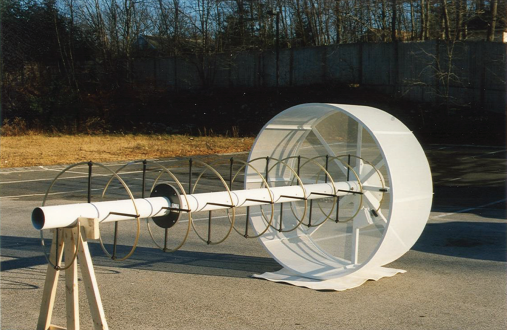
\includegraphics[width=0.60\textwidth]{helical_balanis.png}
	\caption{Hélice comercial con un plano de tierra ahuecado}
	\label{fig:helical_balanis}
\end{figure}

\newpage
\bibliographystyle{plain}
\bibliography{biblist}
\newpage

\printglossary[type=\acronymtype]

\newpage
\printglossary[type=main]

\end{document}